\begin{frame}{What is the problem?}{Motivation}
    \begin{center}
        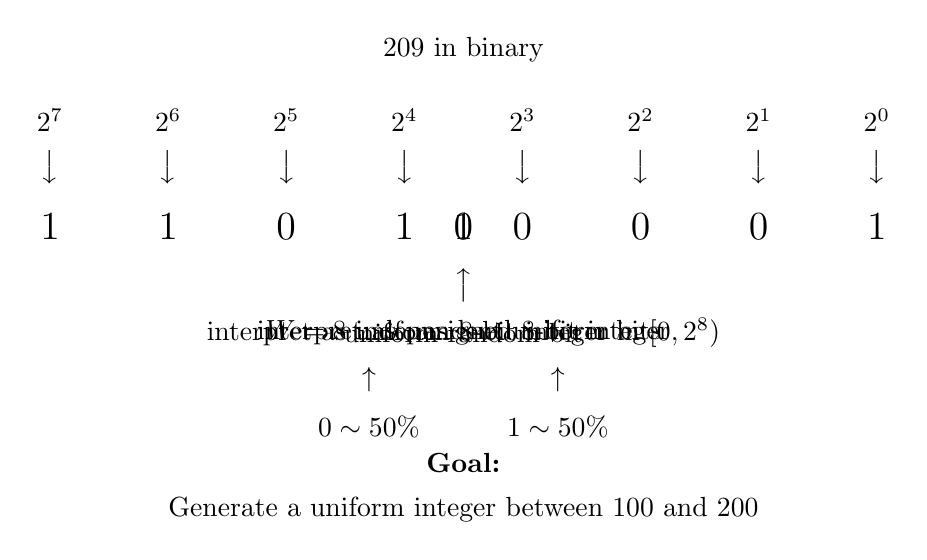
\begin{tikzpicture}[scale = 1.5]
            % One Bit
            \node<1> at (5.0,0.0) {\Large{$0$}};
            \node<2-4> at (5.0,0.0) {\Large{$1$}};
            \node<3-4> at (5.0,-0.5) {$\big\uparrow$};
            \node<3-4> at (5.0,-0.9) {uniform random bit};
            \node<4> at (4.2,-1.3) {$\uparrow$};
            \node<4> at (5.8,-1.3) {$\uparrow$};
            \node<4> at (4.2,-1.7) {$0 \sim 50\%$};
            \node<4> at (5.8,-1.7) {$1 \sim 50\%$};

            % Multiple Bits
            \node<5-> at (1.5,0.0) {\Large{$1$}};
            \node<5-> at (2.5,0.0) {\Large{$1$}};
            \node<5-> at (3.5,0.0) {\Large{$0$}};
            \node<5-> at (4.5,0.0) {\Large{$1$}};
            \node<5-> at (5.5,0.0) {\Large{$0$}};
            \node<5-> at (6.5,0.0) {\Large{$0$}};
            \node<5-> at (7.5,0.0) {\Large{$0$}};
            \node<5-> at (8.5,0.0) {\Large{$1$}};

            \node<6-7> at (5.0,-0.9) {$W = 8$ independent uniform bits};
            \node<7-> at (5.0,-2.0) {\GB{\textbf{Goal:}}};
            \node<7-> at (5.0,-2.4) {Generate a uniform integer between $100$ and $200$};

            \node<8-13> at (5.0,-0.9) {\GB{interpret} as unsigned $8$-bit integer};
            \node<14> at (5.0,-0.9) {\GB{interpret} as uniform $8$-bit integer in $[0,2^8)$};

            \node<9-> at (8.5,0.5) {$\big\downarrow$};
            \node<9-> at (8.5,0.9) {$2^0$};
            \node<10-> at (7.5,0.5) {$\big\downarrow$};
            \node<10-> at (7.5,0.9) {$2^1$};
            \node<11-> at (6.5,0.5) {$\big\downarrow$};
            \node<11-> at (6.5,0.9) {$2^2$};
            \node<12-> at (5.5,0.5) {$\big\downarrow$};
            \node<12-> at (5.5,0.9) {$2^3$};
            \node<12-> at (4.5,0.5) {$\big\downarrow$};
            \node<12-> at (4.5,0.9) {$2^4$};
            \node<12-> at (3.5,0.5) {$\big\downarrow$};
            \node<12-> at (3.5,0.9) {$2^5$};
            \node<12-> at (2.5,0.5) {$\big\downarrow$};
            \node<12-> at (2.5,0.9) {$2^6$};
            \node<12-> at (1.5,0.5) {$\big\downarrow$};
            \node<12-> at (1.5,0.9) {$2^7$};

            \node<13-> at (5.0,1.5) {$209$ in binary};

            \node[opacity=0] at (5.0,1.5) {$209$ in binary};
        \end{tikzpicture}
    \end{center}
\end{frame}